\documentclass{beamer}
\usepackage{listings}
\usepackage{color}
\usepackage{amsmath}
\usepackage{gvv}

\title{Application Problem}
\author{EE25BTECH11008 - Anirudh M Abhilash}
\date{October 4, 2025}

\begin{document}

%----------------- Title -------------------
\begin{frame}
\titlepage
\end{frame}

%----------------- Problem -------------------
\begin{frame}{Problem Statement}
A fraction becomes $\frac{1}{3}$ when $1$ is subtracted from the numerator and it becomes $\frac{1}{4}$ when $8$ is added to the denominator. Find the fraction.
\end{frame}

%----------------- Solution -------------------
\begin{frame}{Solution}
\begin{align}
\frac{x-1}{y} &= \frac{1}{3}, \\
\frac{x}{y+8} &= \frac{1}{4}
\end{align}

\begin{align}
3(x-1) - y &= 0 \implies 3x - y - 3 = 0, \\
4x - (y+8) &= 0 \implies 4x - y - 8 = 0
\end{align}

\begin{align}
(3 \ -1) \myvec{x \\ y} &= 3, \\
(4 \ -1) \myvec{x \\ y} &= 8
\end{align}
\end{frame}

%----------------- Solution (cont) -------------------
\begin{frame}{Solution (cont..)}
Augmented matrix:

\begin{align}
\augvec{2}{1}{3 & -1 & 3 \\ 4 & -1 & 8}
\end{align}

RREF using row operations:

\begin{align}
R_2 &\to R_2 - \frac{4}{3} R_1 \implies 
\augvec{2}{1}{3 & -1 & 3 \\ 0 & 1/3 & 4} \implies
\augvec{2}{1}{3 & -1 & 3 \\ 0 & 1 & 12}, \\
R_1 &\to R_1 + R_2 \implies 
\augvec{2}{1}{3 & 0 & 15 \\ 0 & 1 & 12} \implies
\augvec{2}{1}{1 & 0 & 5 \\ 0 & 1 & 12}
\end{align}
\end{frame}

%----------------- Solution (cont) -------------------
\begin{frame}{Solution (cont..)}
\begin{align}
\myvec{x \\ y} = \myvec{5 \\ 12}
\end{align}

Hence, the fraction is:

\[
\boxed{\frac{5}{12}}
\]
\end{frame}

\begin{frame}[fragile]{Python Code (Plotting Line and Vectors)}
\begin{lstlisting}[language=Python]
import numpy as np
import matplotlib.pyplot as plt

m1, c1 = 1.5, 2 
m2, c2 = -0.5, 5     
A = np.array([0, c1])
B = np.array([0, c2])
x_intersect = (c2 - c1) / (m1 - m2)
y_intersect = m1 * x_intersect + c1
C = np.array([x_intersect, y_intersect])
triangle = np.array([A, B, C, A]) 
\end{lstlisting}
\end{frame}

\begin{frame}[fragile]{Python Code (cont..)}
\begin{lstlisting}[language=Python]
plt.figure(figsize=(6,6))
plt.plot(triangle[:,0], triangle[:,1], 'b-o', label='Triangle')
plt.axvline(0, color='k', linewidth=0.8) 
plt.axhline(0, color='k', linewidth=0.8) 
x_vals = np.linspace(min(0, C[0])-1, max(C[0]+1, 2), 100)
plt.plot(x_vals, m1*x_vals + c1, 'r--', label=f'y={m1}x+{c1}')
plt.plot(x_vals, m2*x_vals + c2, 'g--', label=f'y={m2}x+{c2}')
\end{lstlisting}
\end{frame}

\begin{frame}[fragile]{Python Code (cont..)}
\begin{lstlisting}[language=Python]
plt.scatter([A[0], B[0], C[0]], [A[1], B[1], C[1]], color='black')
plt.text(A[0]-0.3, A[1]+0.1, 'A')
plt.text(B[0]-0.3, B[1]+0.1, 'B')
plt.text(C[0]+0.1, C[1]+0.1, 'C')
plt.grid(True)
plt.axis('equal')
plt.title('Triangle formed by lines and x=0')

plt.show()
\end{lstlisting}
\end{frame}

%----------------- Plot -------------------
\begin{frame}[fragile]{Plot}
\begin{figure}[H]\centering
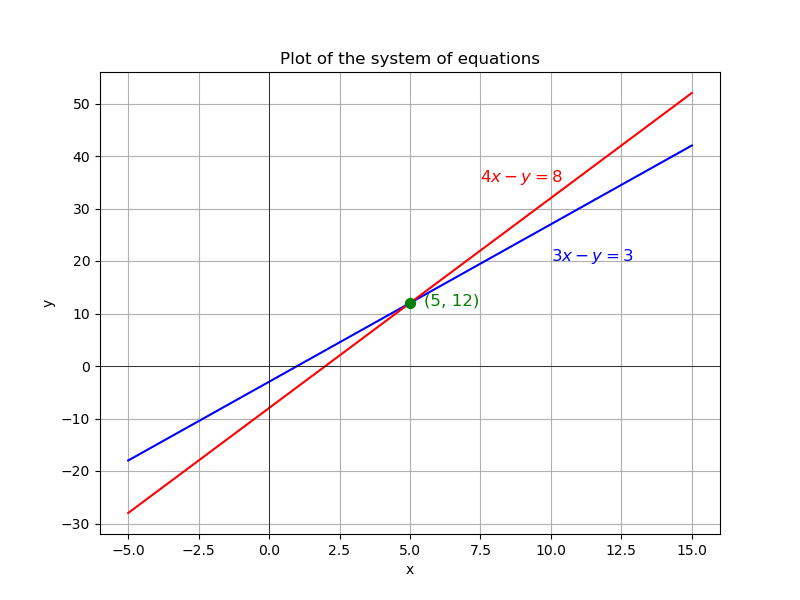
\includegraphics[width=1\columnwidth]{figs/plt.png}
\caption{Triangle with example points}
\label{fig:plt}
\end{figure}
\end{frame}

%----------------- C Code -------------------

\begin{frame}[fragile]{C Code (Computations)}
\begin{lstlisting}[language=C]
#include <stdio.h>

void get_lines(double* x, double* y1, double* y2, int n) {
    for (int i = 0; i < n; i++) {
        y1[i] = 3*x[i] - 3.0; 
        y2[i] = 4*x[i] - 8.0; 
    }
}
\end{lstlisting}
\end{frame}

%----------------- Python Code -------------------
\begin{frame}[fragile]{Python Code (Using C)}
\begin{lstlisting}[language=Python]
import numpy as np
import matplotlib.pyplot as plt
import ctypes

lines_lib = ctypes.CDLL('./points.so')

n = 100
x = np.linspace(-5, 15, n)
y1 = np.zeros(n, dtype=np.float64)
y2 = np.zeros(n, dtype=np.float64)
\end{lstlisting}
\end{frame}

\begin{frame}[fragile]{Python Code (Cont..)}
\begin{lstlisting}[language=Python]
lines_lib.get_lines.argtypes = [
    np.ctypeslib.ndpointer(dtype=np.float64, ndim=1, flags="C_CONTIGUOUS"),
    np.ctypeslib.ndpointer(dtype=np.float64, ndim=1, flags="C_CONTIGUOUS"),
    np.ctypeslib.ndpointer(dtype=np.float64, ndim=1, flags="C_CONTIGUOUS"),
    ctypes.c_int
]
lines_lib.get_lines(x, y1, y2, n)

plt.figure(figsize=(8, 6))
plt.plot(x, y1, color='blue')
plt.plot(x, y2, color='red')
\end{lstlisting}
\end{frame}

\begin{frame}[fragile]{Python Code (Cont..)}
\begin{lstlisting}[language=Python]
plt.text(10, 20, r'$3x - y = 3$', color='blue', fontsize=12)
plt.text(7.5, 35, r'$4x - y = 8$', color='red', fontsize=12)

plt.title("System of Equations")
plt.xlabel("x")
plt.ylabel("y")
plt.grid(True)
plt.axhline(0, color='black', linewidth=0.5)
plt.axvline(0, color='black', linewidth=0.5)
plt.show()
\end{lstlisting}
\end{frame}

\end{document}